\documentclass{article}
\usepackage{graphicx}
\usepackage{listings}
\usepackage{float}
\usepackage{url}
\usepackage[numbers]{natbib}
\usepackage{color} %red, green, blue, yellow, cyan, magenta, black, white
\definecolor{mygreen}{RGB}{28,172,0} % color values Red, Green, Blue
\definecolor{mylilas}{RGB}{170,55,241}


\begin{document}

\lstset{language=Matlab,%
    %basicstyle=\color{red},
    breaklines=true,%
    morekeywords={matlab2tikz},
    keywordstyle=\color{blue},%
    morekeywords=[2]{1}, keywordstyle=[2]{\color{black}},
    identifierstyle=\color{black},%
    stringstyle=\color{mylilas},
    commentstyle=\color{mygreen},%
    showstringspaces=false,%without this there will be a symbol in the places where there is a space
    numbers=left,%
    numberstyle={\tiny \color{black}},% size of the numbers
    numbersep=9pt, % this defines how far the numbers are from the text
    emph=[1]{for,end,break},emphstyle=[1]\color{red}, %some words to emphasise
    %emph=[2]{word1,word2}, emphstyle=[2]{style},
}

\section{Requirement 1 : Correlation Detector}

Simple correlation can be performed using a template and image,
all tests in this report used the obama.png as the template image. The results of
using a simple correlation can be seen in figure \ref{fig:simplecor}. As can be
seen this results is significant numbers of false positive detections, expecially
in the flag section above the rows of people. Also many detections are not successfully
centered around the face.\\

\begin{figure}[H]
  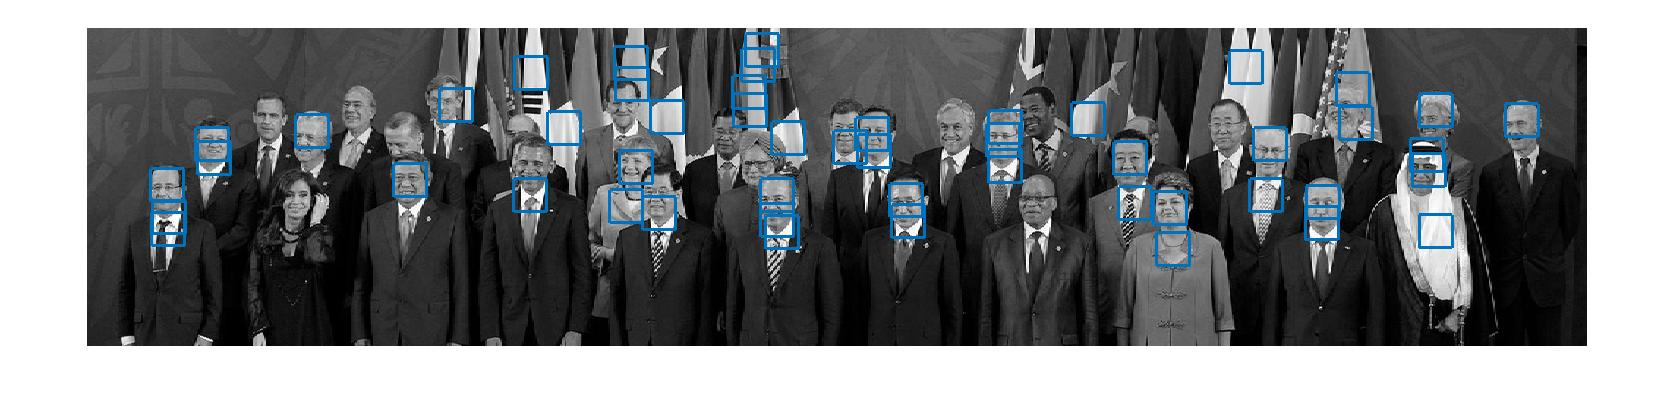
\includegraphics[width=\linewidth]{simpleCor.jpg}
  \caption{Results of using Simple Correlation on g20 image}
  \label{fig:simplecor}
\end{figure}

To improve this a normalised correlation technique was implemented. The normalised correlation
is defined in the coursework specification and is shown in figure \ref{fig:normcoreq} for reference.
This can be simplified in a series of steps to make use of correlations in order to
improve performance. Firstly the value of $x - m_x1$ can be precomputed as this is
simply the template minus its mean. Next the numerator of the fraction can be expanded
to give $xy + m_x1m_y1 - xm_y1 - ym_x1$, each of these four terms can then be computed
using a correlation. These four correlations are shown in figure \ref{fig:numerator}
where template and image are the vectorised image and template, templateMean is
the mean of the template and imageMean is a matrix of the mean values at each template
location. imageMean can be computed using another correlation with a template of values 1/1024 where
the template size is 32 x 32.\\

\begin{figure}[H]
\begin{center}
$r=\frac{(x-m_x1)^T(y-m_y1)}{|x-m_x1||y-m_x1|}$
\end{center}
\caption{Normalised Correlation}
\label{fig:normcoreq}
\end{figure}

\begin{figure}[H]
\begin{lstlisting}
MxY = filter2(templateMean, image);
XMy = filter2(template, imageMean);
MxMy = filter2(templateMean, imageMean);
XY = filter2(template, image);
\end{lstlisting}
\caption{Numerator Compute Code}
\label{fig:numerator}
\end{figure}

Now the numerator of the normalised correlation is computed we can turn to the
denominator. The denominator of the normalised correlation equation is the
standard deviation of the template multiplied by the standard deviation of the part of the image under the template \cite{crosscor}.
The standard deviation of the template can be computed using std(). The standard
deviation of the part of the image under the tempalte is more difficult to compute. The standard deviation can be
rearranged to the equation shown in figure \ref{fig:stddeveq} where n is the
number of pixels under the template, q is the squared sum of the pixels under the
template and s is the sum of the pixels under the template \cite{stddev}. This can
be computed using another three correlations to compute n, q and s as shown in
figure \ref{fig:stddeccode} where the template is of size 32 x 32.\\

\begin{figure}[H]
\begin{center}
$r=\frac{1}{n - 1}(q - \frac{s^2}{n})$
\end{center}
\caption{Standard Deviation}
\label{fig:stddeveq}
\end{figure}

\begin{figure}[H]
\begin{lstlisting}[language=matlab]
n = filter2(ones(size(32, 32), ones(32, 32), 'same');

imSquared = im .^2;
q = filter2(ones(32, 32), imSquared, 'same');

s = filter2(32, 32, image, 'same');

imStdDev = (q - ((s .^ 2) ./ n) ./ (n - 1));

imStdDev = sqrt(imStdDev);
\end{lstlisting}
\caption{Standard Deviation matlab}
\label{fig:stddeccode}
\end{figure}

Using the normalised correlation the output of the face detection using obama.png
as the template is shown in figure \ref{fig:normalisedcor}. As can be seen there
is still a high number of false detections in the background of the image as well
as in the tie area of some people. The next section will try and address these issues
with an improved detector.\\

\begin{figure}[H]
  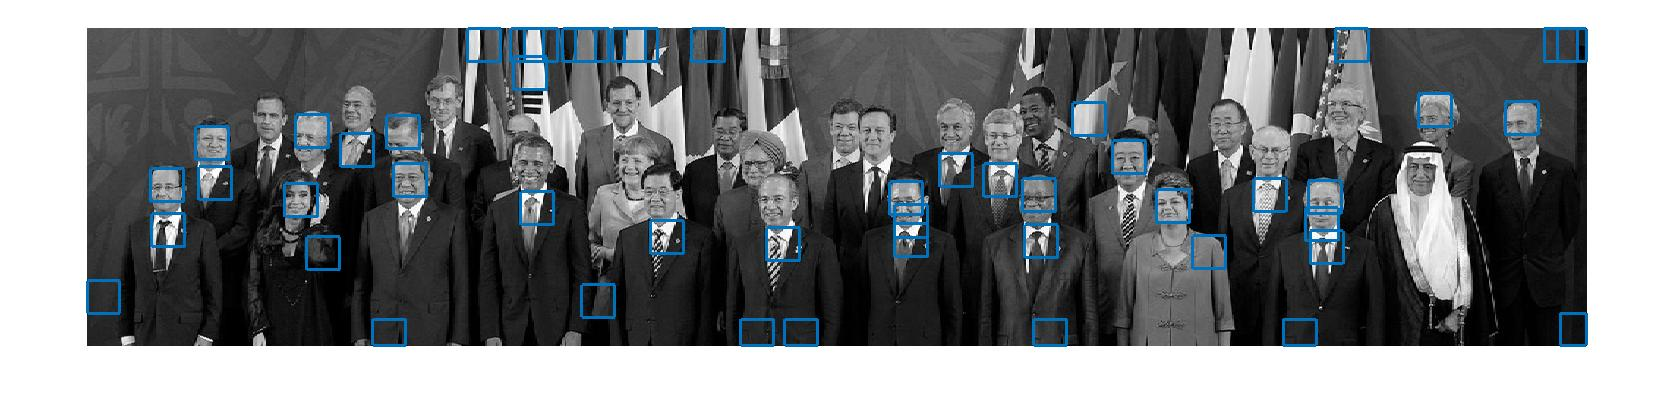
\includegraphics[width=\linewidth]{normalisedCor.jpg}
  \caption{Results of using Normalised Correlation on g20 image}
  \label{fig:normalisedcor}
\end{figure}

\section{Requirement 2 : Improved Detector}

The original normalised correlation detector achieves 27\% overlap with the Viola-Jones
face detection algorithm and this will be used as the performance measures for
the improvements demonstrated in this section.\\

\subsection{Guassian Blur}

One improvement which was tried was to add a Gaussian blur using a correlation of
a Gaussian template. The idea here was to remove some of the fine grain detain and
high frequencies in the template image as these high frequencies may be causing
some of the missed faces. This did increase the overlap to 29\% the result can
be seen in figure \ref{fig:blurred}. The number of correctly detected faces is
improved however there are still high numbers of false positives.\\

\begin{figure}[H]
  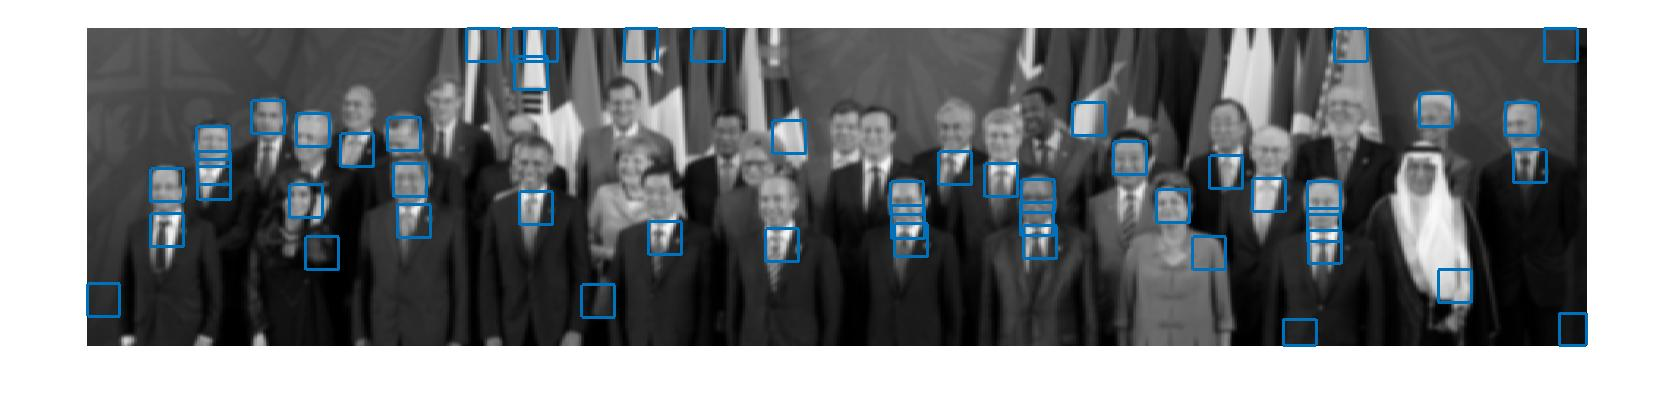
\includegraphics[width=\linewidth]{blurred.jpg}
  \caption{Results of using Normalised Correlation and Guassian Blur on g20 image}
  \label{fig:blurred}
\end{figure}

\subsection{Colour Filtering}

As many of the false detections are caused in the background of the image where
the colours are not similar to skin tones a colour filter was implemented to try
and reduce their occurrence. Using the training data supplied the upper and lower
bounds for skin tone colours in red, green and blue where found. Any pixel which
did not fall within these bounds was set to black. It was found that only applying
the colour filter to the g20 image and not the template caused highest nubmers of
detections. This achived an overlap of 50\%, which is shown in figure \ref{fig:colourfilt}.
As can be seen in the figure there are significantly less false detections in the
background of the image and also more correct detections as a result of reducing
the search space down to the pixels which are within skin tone ranges.\\

\begin{figure}[H]
  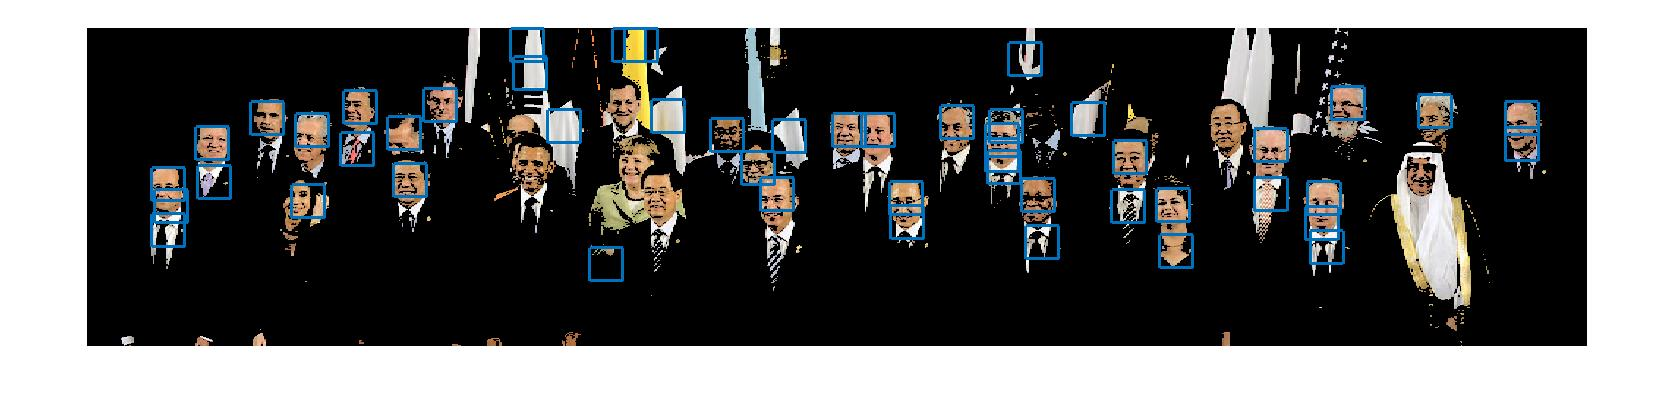
\includegraphics[width=\linewidth]{colourfilt.jpg}
  \caption{Results of using Normalised Correlation and Colour Filter on g20 image}
  \label{fig:colourfilt}
\end{figure}

\subsection{Edge Detection}

The final improvement on the original normalised correlation technique was using
edge detection. The idea behind this was to simplfy the image down to just an edge
detected image this means that the detection is just using the shape of the edges
in the image as opposed to the colour or grayscale pixel value. It was expected
that this would reduce the number of false detection is the background as the edges
here are simple verticle lines which are not similar to those in the tempalate image.
It was also expected that the number of correct detections would increase as the grey
scale values are no longer being compared, so skin tone should not be an issue.\\

In order to create an edge detected image the Canny edge detection technique was
applied. Firstly the Sobel Kernels are applied in two
convolutions, for the horizontal and vertical. After this the gradients at each pixel
are computed and are set to the closest of the two diagonals, horizontal and vertical.
Finally the values are all thresholded to only leave the hard edges.\\

Using the edge detected image an overlap of 34\% was achieved, this is shown in
figure \ref{fig:edgedet}. As expected the number of false detections in the background
of the image is reduced compared to the original normalised correlation and there
are more positive detections.

\begin{figure}[H]
  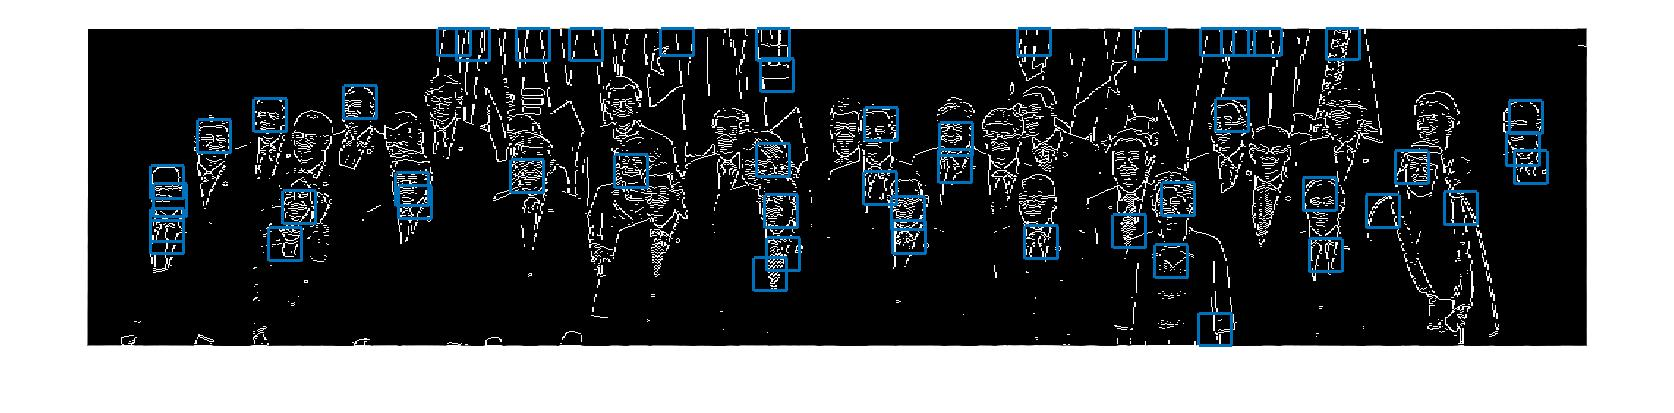
\includegraphics[width=\linewidth]{edgedetect.jpg}
  \caption{Results of using Normalised Correlation and Edge Detection on g20 image}
  \label{fig:edgedet}
\end{figure}

\subsection{Harr Features}

The final detection technique which was tried was to move away from using a convolution
of a template image and to use Harr features like the Viola-Jones algorithm does \cite{viola2004robust}.
The Viola-Jones algorithm uses a cascade of simple classifiers using a Harr feature
to detect faces. Therefore the use of a set Harr features to detect an face should yeild
an improved overlap with the Viola-Jones algorithm.\\

In order to do this a seven Harr Features were used each of a fixed size, these
were chosen by running all possible sizes of the two, three and four segment Harr
features over a test set of faces and non faces. The features which gave the highest
success rate when run on the test set were used in the final implementation. An
integral image of the target image is created in order to compare the Harr features
too. Each of the Harr features were used as the template for a convolution across the
Wintegral image. The average of each pixel in each convolution is calculated giving an
matrix where high values represent where more of the Harr features matched the image below.
An example of the output when run on the g20 image is shown in figure \ref{fig:harrfeat},
as can be seen lighter areas are where faces are in the image. This technique yeilds
a 49\% overlap with the Viola-Jones algorithm.

\begin{figure}[H]
  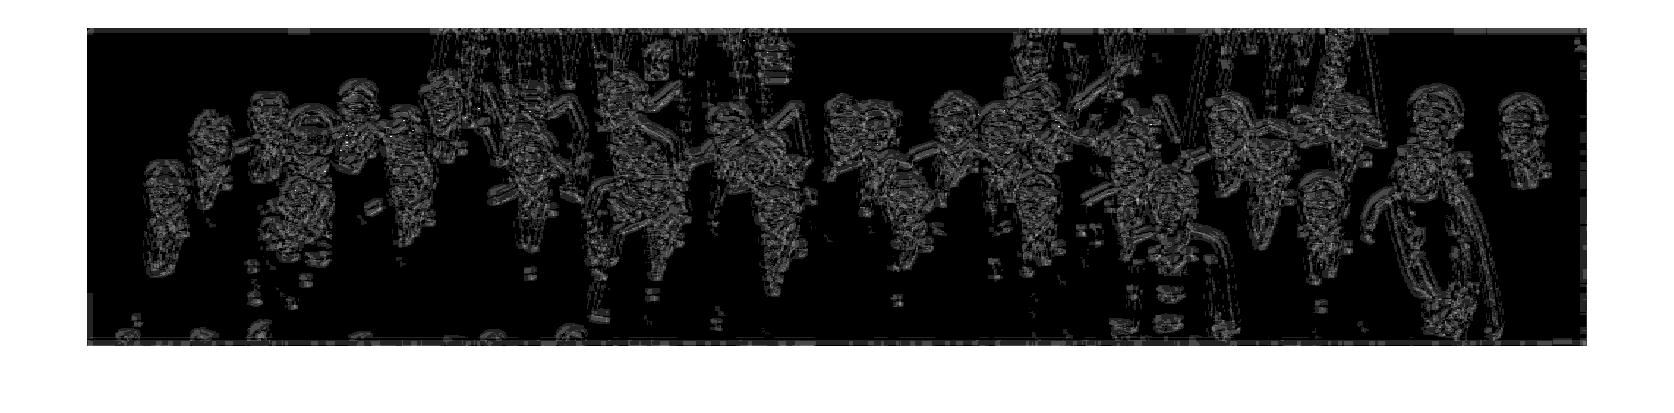
\includegraphics[width=\linewidth]{harrfeat.jpg}
  \caption{Results of using Harr feature technique on g20 image}
  \label{fig:harrfeat}
\end{figure}

\section{Requirement 3 : Nearest-Neighbour Classifier}

In order to create a nearest-neighbour style classifier the euclidean distance
between each of the detected face and the faces in the database are computed.
Firstly each image in the database and the extracted images has its mean subtracted
and is divided by its standard deviation in order to normalise lighting conditions.
The euclidean distance is simply the squared distance between each pixel value
in two images summed together. For each extracted image the distance between each
image in the database is computed and the database image with the smallest distance
is recorded and the class that image belongs to is the person that extraction is
classified as. The code for this is in the EuclideanClassifier.m file.\\

Using this classifier 5 out of the 18 faces which are extracted by the face detection
algorithm are correctly classified. This gives an overall success rate of 28\%.
This is shown in figure \ref{fig:nnc}.

\begin{figure}[H]
  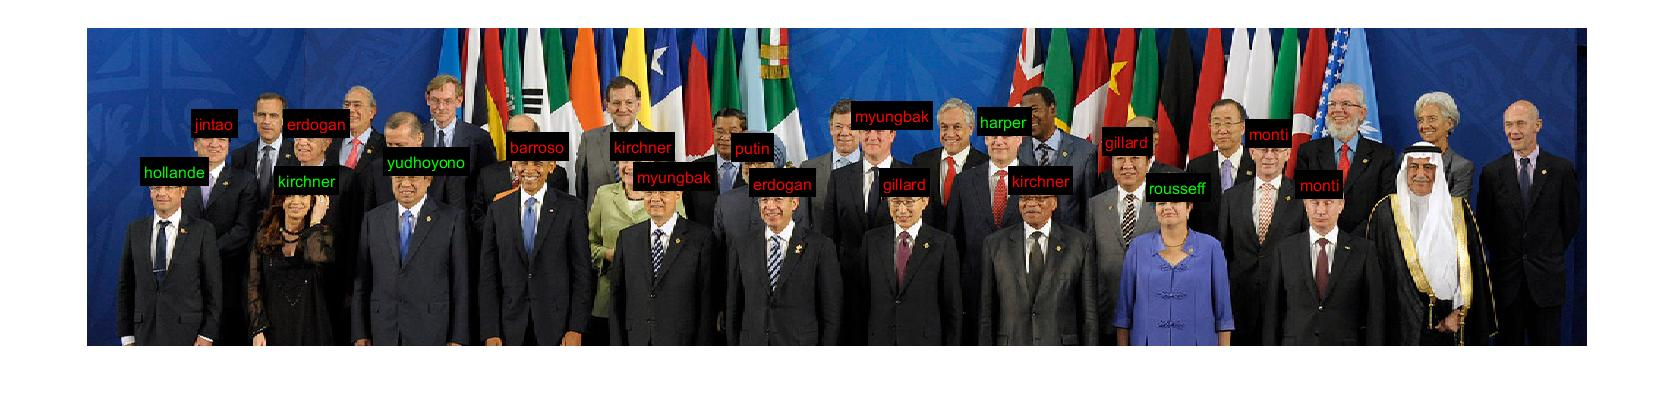
\includegraphics[width=\linewidth]{euclidean.jpg}
  \caption{Results of face classification using Nearest-Neighbour Classifier}
  \label{fig:nnc}
\end{figure}

\section{Requirement 4 : Improved Classifier}

\subsection{Using SVM and Naive Bayes classifiers}

The first improvement which was tried was to replace the Nearest-Neighbour classifier
with a different classifier. Two classifiers were tried first a Support Vector Machine
and then a Naive Bayes classifier. Feature vectors for both classifiers are simply
vectorised versions of the 32 x 32 images. The SVM approach comprises of a binary SVM for
each of the classes of image. Each singe classifier returns true or false depending
on whether the image passed is classified as the class the SVM was trained of.
Each SVM is trained using all images of the face it is to classify as class True
and all other faces in the database as class False. Then in order to classify am
unknown face each SVM is run in turn until one returns true. The Naive Bayes approach
uses a multi class Naive Bayes trained on the database of images provided.\\

Both of these classifiers produced very similar success rates of 28\% for the SVM
and 22\% for the Naive Bayes these are no better than the Nearest-Neighbour classifier.
It was decided to change the features used in the classification next as opposed to
modifying any of the classifiers parameters.\\

\subsection{Using Eigen Faces}

Eigen faces can be used as a feature for a face classifier. In order to create a
set of eigen faces from the database firstly the average image is computed, the
left most image in figure \ref{fig:eigenface}. The eigen faces are then computed
by eigen value decomposition, each of the training images is placed in a M x N
matrix where M is the number of images and N there vectorised length. The convolution
matrix of this is then computed giving a N x N matrix, the eigen vectors of this
are the eigen faces \cite{eigface}. Each eigen face is normalised between 0 and 1. The first
five eigen faces are shown in figure \ref{fig:eigenface}.\\

\begin{figure}[H]
  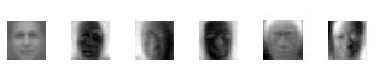
\includegraphics[width=\linewidth]{eigenface.jpg}
  \caption{Average Face and largest Eigen Faces, Left to Right}
  \label{fig:eigenface}
\end{figure}

After the eigen faces have been computed then can be used to build feature vectors
for images. This is done by computing the weights required for each of the eigen
faces in order to reproduce the image. The weights are created by firstly taking
the average face away from the target image then computing the dot product
between each eigen face giving the weight for that eigen face. This gives a vector
who's length is the same as the number of eigen faces, and can be used as a feature
vector for face classification.\\

Using a set of training and testing data from the database it was found that the
optimum eigen faces to use were the 50 largest. It was also found that a Naive Bayes
classifier yielded the highest success rate. Using a naive bayes classifier trained with
the weights for each of the images in the database and then run against the faces
extracted by the Viola-Jones algorithm a success rate of 56% was achieved, which is
significantly better than the nearest neighbor approach. The results are shown in
figure \ref{fig:eigenfaces}.

\begin{figure}[H]
  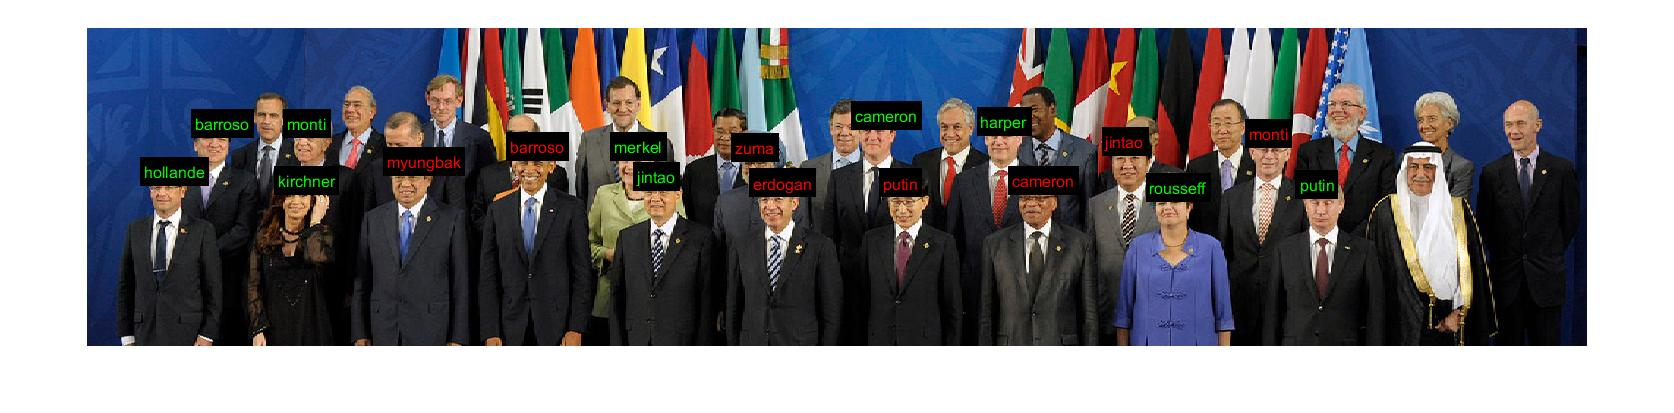
\includegraphics[width=\linewidth]{eigenfacesrun.jpg}
  \caption{Results of face classification using Eigen Faces}
  \label{fig:eigenfaces}
\end{figure}


\bibliographystyle{acm}
\bibliography{report}

\end{document}
